\newpage
\subsection{Esercizio 16}
Eseguendo \nameref{cod:16} si ottiene:
\begin{figure}[h!]
    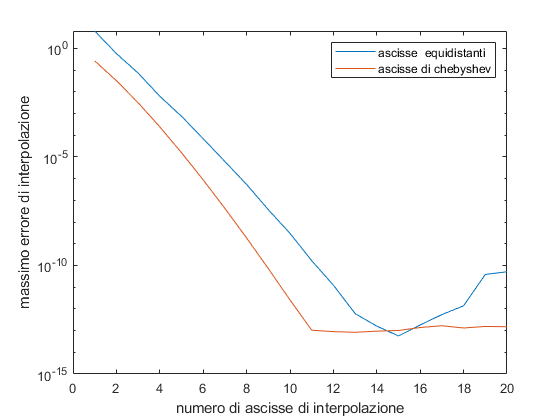
\includegraphics[scale=0.8]{capitolo4/hermite.png}
    \caption{risultati interpolazione hermite}
    \label{fig:16}
\end{figure}


Si può notare come, rispetto all'interpolazione classica, l'errore decresca più rapidamente per $n \le 15$. Anche in questo caso l'errore commesso usando le ascisse di chebyshev
è migliore in confronto al caso delle ascisse equidistanti(eccetto per $n=15$).